\documentclass[11pt]{article}\usepackage[]{graphicx}\usepackage[usenames,dvipsnames]{xcolor}
% maxwidth is the original width if it is less than linewidth
% otherwise use linewidth (to make sure the graphics do not exceed the margin)
\makeatletter
\def\maxwidth{ %
  \ifdim\Gin@nat@width>\linewidth
    \linewidth
  \else
    \Gin@nat@width
  \fi
}
\makeatother

\definecolor{fgcolor}{rgb}{0.345, 0.345, 0.345}
\newcommand{\hlnum}[1]{\textcolor[rgb]{0.686,0.059,0.569}{#1}}%
\newcommand{\hlstr}[1]{\textcolor[rgb]{0.192,0.494,0.8}{#1}}%
\newcommand{\hlcom}[1]{\textcolor[rgb]{0.678,0.584,0.686}{\textit{#1}}}%
\newcommand{\hlopt}[1]{\textcolor[rgb]{0,0,0}{#1}}%
\newcommand{\hlstd}[1]{\textcolor[rgb]{0.345,0.345,0.345}{#1}}%
\newcommand{\hlkwa}[1]{\textcolor[rgb]{0.161,0.373,0.58}{\textbf{#1}}}%
\newcommand{\hlkwb}[1]{\textcolor[rgb]{0.69,0.353,0.396}{#1}}%
\newcommand{\hlkwc}[1]{\textcolor[rgb]{0.333,0.667,0.333}{#1}}%
\newcommand{\hlkwd}[1]{\textcolor[rgb]{0.737,0.353,0.396}{\textbf{#1}}}%
\let\hlipl\hlkwb

\usepackage{framed}
\makeatletter
\newenvironment{kframe}{%
 \def\at@end@of@kframe{}%
 \ifinner\ifhmode%
  \def\at@end@of@kframe{\end{minipage}}%
  \begin{minipage}{\columnwidth}%
 \fi\fi%
 \def\FrameCommand##1{\hskip\@totalleftmargin \hskip-\fboxsep
 \colorbox{shadecolor}{##1}\hskip-\fboxsep
     % There is no \\@totalrightmargin, so:
     \hskip-\linewidth \hskip-\@totalleftmargin \hskip\columnwidth}%
 \MakeFramed {\advance\hsize-\width
   \@totalleftmargin\z@ \linewidth\hsize
   \@setminipage}}%
 {\par\unskip\endMakeFramed%
 \at@end@of@kframe}
\makeatother

\definecolor{shadecolor}{rgb}{.97, .97, .97}
\definecolor{messagecolor}{rgb}{0, 0, 0}
\definecolor{warningcolor}{rgb}{1, 0, 1}
\definecolor{errorcolor}{rgb}{1, 0, 0}
\newenvironment{knitrout}{}{} % an empty environment to be redefined in TeX

\usepackage{alltt}
\usepackage[sc]{mathpazo} %Like Palatino with extensive math support
\usepackage{fullpage}
\usepackage[authoryear,sectionbib,sort]{natbib}
\linespread{1.7}
\usepackage[utf8]{inputenc}
\usepackage{lineno}
\usepackage{titlesec}
\titleformat{\section}[block]{\Large\bfseries\filcenter}{\thesection}{1em}{}
\titleformat{\subsection}[block]{\Large\itshape\filcenter}{\thesubsection}{1em}{}
\titleformat{\subsubsection}[block]{\large\itshape}{\thesubsubsection}{1em}{}
\titleformat{\paragraph}[runin]{\itshape}{\theparagraph}{1em}{}[. ]\renewcommand{\refname}{Literature Cited}
% my addnl packages
\usepackage{geometry}
\usepackage{graphicx}
\usepackage[T1]{fontenc}
\usepackage[utf8]{inputenc}
\usepackage{authblk}
\usepackage{setspace}
\usepackage{amsfonts,amssymb,amsmath,hyperref}
\usepackage{float}
\usepackage{caption}
\usepackage{multirow}
\usepackage{hyperref}
\usepackage{wrapfig}
\usepackage{rotating}
\usepackage[usenames,dvipsnames]{xcolor}
\newcommand{\revise}[1]{{\color{Mahogany}{#1}}}
\usepackage[normalem]{ulem}
\newcommand{\tom}[2]{{\color{red}{#1}}\footnote{\textit{\color{red}{#2}}}}

\doublespacing
%\bibliography{creosote_SIPM}



\title{Appendix S3}
\author{Trevor H., Drees, Brad M. Ochocki, Scott L. Collins, and T.E.X. Miller}
\date{\vspace{-5ex}}
\IfFileExists{upquote.sty}{\usepackage{upquote}}{}
\begin{document}
\maketitle
\noindent{} \textbf{Demography and dispersal at a grass-shrub ecotone: a spatial integral projection model for woody plant encroachment. \textit{Ecological Monographs}}

\renewcommand{\thefigure}{S\arabic{figure}}\setcounter{figure}{0}
\renewcommand{\thetable}{S\arabic{table}}\setcounter{table}{0}
\renewcommand{\theequation}{S\arabic{equation}}\setcounter{equation}{0}

We censused transplant survival twice following July 2015 planting, in fall 2015 and spring 2016. 
Here, we analyze the two survival intervals separately, including grass and shrub cover at the local ($1m$x$1m$) scale as explanatory variables in addition to the weighted density of the 5-m transect window as presented in the main text. 

For both fall and spring survival censuses, we fit eight candidate models that included all combinations of window weighted density, local shrub cover (proportion of plot area covered by creosotebush), and local grass cover (proportion of plot area covered by any grass species) as smooth terms in a generalized additive model.
We used a binomial response distribution where ``successes'' were the number of survivors per plot and ``trials'' were the number of seedlings planted for fall survival (always four per plot) and the number of fall survivors for spring survival. 
All models included a random effect of transect. 
We used AIC-based model selection to quantify support for competing models. 

\paragraph{Results}The majority of mortality occurred within the first census interval (53 fall survivors out of 576 transplants), resulting in a much smaller data set for the second census interval (20 spring survivors out of 53 fall survivors).

For fall survival, the top model (Model 7) included effects of creosotebush weighted density at the 5-m window scale and local grass cover (Table \ref{tab:fall_aic}). 
Fall survival was low overall but greatest in zero-density windows and there was a weak negative effect of local grass cover (Figure \ref{fig:survapp}).
Three additional models (2, 5 and 8) were within 2 AIC units of the top model (Table \ref{tab:fall_aic}). 
Despite the model uncertainty, these top four models included shrub weighted density and comprised \>87\% of AIC weight, providing strong support for negative effects of shrub density at the scale of 5-m windows, consistent with the full analysis (transplant experiment + observational census) presented in the main text.

Spring survival was dominated by high model uncertainty, and the most complex model (8) did not converge due to inadequate data. 
The top-ranked model was Model 6, which included effects of local shrub and grass cover.
However, the null model (1) was nearly tied with the top model, and six of seven models were within 2 AIC units. 
Given the relatively small data set, a conservative interpretation is that there is not sufficient evidence to reject the null hypothesis of a constant fall-to-spring survival rate that was unrelated to shrub or grass density. 

% latex table generated in R 4.2.2 by xtable 1.8-4 package
% Tue Mar 28 11:42:48 2023
\begin{table}[ht]
\centering
\begin{tabular}{|p{12cm}|c|c|}
  \hline
Pr(Survival) & df & dAIC \\ 
  \hline
(1$|$transect) & 8.93 & 11.98 \\ 
  window density + (1$|$transect) & 9.97 & 0.49 \\ 
  shrub cover + (1$|$transect) & 10.82 & 3.51 \\ 
  grass cover + (1$|$transect) & 11.02 & 6.65 \\ 
  window density + shrub cover + (1$|$transect) & 12.11 & 1.04 \\ 
  grass cover + shrub cover + (1$|$transect) & 12.29 & 3.29 \\ 
  window density + grass cover + (1$|$transect) & 11.44 & 0.00 \\ 
  window density + shrub cover + grass cover + (1$|$transect) & 12.39 & 1.80 \\ 
   \hline
\end{tabular}
\caption{AIC model selection for July-October transplant survival probability.} 
\label{tab:fall_aic}
\end{table}


% latex table generated in R 4.2.2 by xtable 1.8-4 package
% Tue Mar 28 11:42:48 2023
\begin{table}[ht]
\centering
\begin{tabular}{|p{12cm}|c|c|}
  \hline
Pr(Survival) & df & dAIC \\ 
  \hline
(1$|$transect) & 1.00 & 0.07 \\ 
  window density + (1$|$transect) & 2.00 & 1.93 \\ 
  shrub cover + (1$|$transect) & 2.00 & 1.22 \\ 
  grass cover + (1$|$transect) & 2.03 & 0.69 \\ 
  window density + shrub cover + (1$|$transect) & 3.00 & 1.85 \\ 
  grass cover + shrub cover + (1$|$transect) & 3.37 & 0.00 \\ 
  window density + grass cover + (1$|$transect) & 3.23 & 2.19 \\ 
   \hline
\end{tabular}
\caption{AIC model selection for October-June transplant survival probability.} 
\label{tab:spring_aic}
\end{table}


\begin{figure}[H]
  \begin{center}
    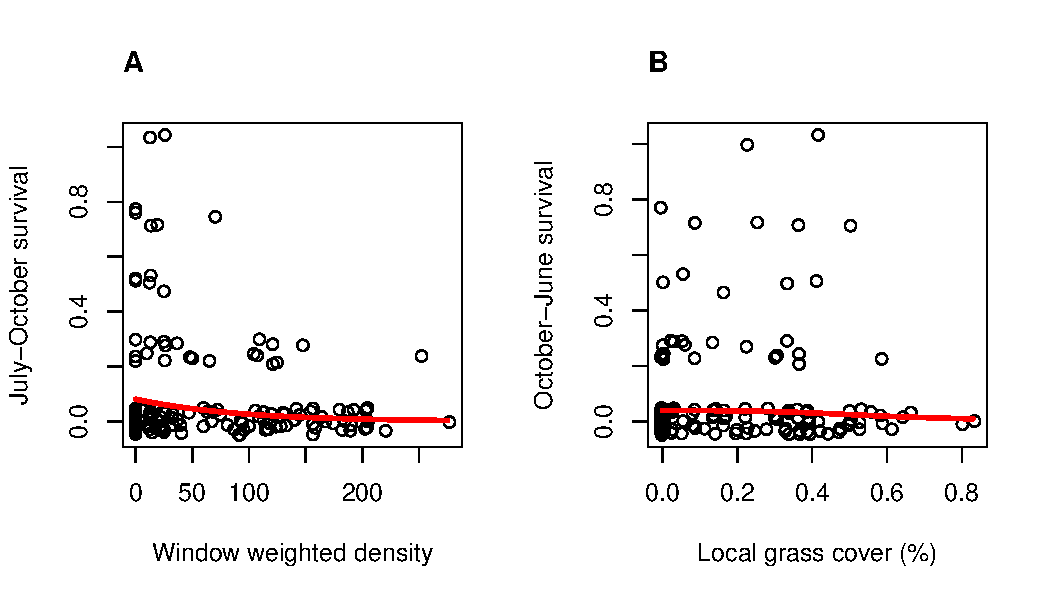
\includegraphics[width=\linewidth]{Figures/SurvivalAppendix}
  \caption{}
  \label{fig:survapp}
  \end{center}
\end{figure}


\end{document}
